\documentclass[sigconf]{acmart}

\usepackage{booktabs} % For formal tables
\usepackage{multirow}
\usepackage{listings}   

\usepackage{tikz}
\usetikzlibrary{automata,positioning}


\lstset{
  frame=none,
  language=scala,
  basicstyle={\small\ttfamily}
}

\sloppy

% Copyright
%\setcopyright{none}
%\setcopyright{acmcopyright}
%\setcopyright{acmlicensed}
\setcopyright{rightsretained}
%\setcopyright{usgov}
%\setcopyright{usgovmixed}
%\setcopyright{cagov}
%\setcopyright{cagovmixed}


% DOI
%\acmDOI{10.475/123_4}

% ISBN
%\acmISBN{123-4567-24-567/08/06}

%Conference
\acmConference[Scala 2018]{Ninth ACM SIGPLAN Symposium on Scala, 2018}{September 2018}{St. Louis, Missouri, United States}
\acmYear{2018}
\copyrightyear{2018}


%\acmArticle{4}
%\acmPrice{15.00}

% These commands are optional
%\acmBooktitle{Transactions of the ACM Woodstock conference}
%\editor{Jennifer B. Sartor}
%\editor{Theo D'Hondt}
%\editor{Wolfgang De Meuter}


\begin{document}
\title{Parser-Combinators for Context-Free Path Querying}
%\titlenote{This work is supported by grant from JetBrains Research.}
%\subtitle{Extended Abstract}
%\subtitlenote{The full version of the author's guide is available as
%  \texttt{acmart.pdf} document}


\author{Sophia Smolina}
\affiliation{%
  \institution{Electrotechnical University}
  \streetaddress{ul. Professora Popova 5,}
  \city{St. Petersburg}
  \country{Russia}
  \postcode{197376}
}
\email{sofysmol@gmail.com}

\author{Ekaterina Verbitskaia}
\affiliation{%
  \institution{Saint Petersburg State University}
  \streetaddress{7/9 Universitetskaya nab.}
  \city{St. Petersburg}
  \country{Russia}
  \postcode{199034}
}
\email{kajigor@gmail.com}

\author{Ilya Kirillov}
\affiliation{%
  \institution{Saint Petersburg State University}
  \streetaddress{7/9 Universitetskaya nab.}
  \city{St. Petersburg}
  \country{Russia}
  \postcode{199034}
}
\email{kirillov.ilija@gmail.com}

\author{Ilya Nozkin}
\affiliation{%
  \institution{Saint Petersburg State University}
  \streetaddress{7/9 Universitetskaya nab.}
  \city{St. Petersburg}
  \country{Russia}
  \postcode{199034}
}
\email{nozhkin.ii@gmail.com}


\author{Semyon Grigorev}
\orcid{0000-0002-7966-0698}
\affiliation{%
  \institution{Saint Petersburg State University}
  \streetaddress{7/9 Universitetskaya nab.}
  \city{St. Petersburg}
  \country{Russia}
  \postcode{199034}
}
\email{s.v.grigoriev@spbu.ru}

% The default list of authors is too long for headers.
\renewcommand{\shortauthors}{Smolina et al.}

\begin{abstract}
A transparent integration of a domain-specific language for specification of context-free path queries (CFPQs) into a general-purpose programming language as well as static checking of errors in queries may greatly simplify the development of applications utilizing CFPQs.  
Such techniques as LINQ and ORM can be used for the integration, but they have issues with flexibility: query decomposition and reusing of subqueries are a challenge.
Adaptation of parser combinators technique for paths querying may solve these problems. 
Conventional parser combinators process linear input and only the Trails library is known to apply this technique for path querying.
Trails suffers the common parser combinators issue: it does not support left-recursive grammars and also experiences problems in cycles handling.
We demonstrate that it is possible to create general parser combinators for CFPQ which support arbitrary context-free grammars and arbitrary input graphs.
We implement a library of such parser combinators and show that it is applicable for realistic tasks.
\end{abstract}

%
% The code below should be generated by the tool at
% http://dl.acm.org/ccs.cfm
% Please copy and paste the code instead of the example below.
%
\begin{CCSXML}
<ccs2012>
<concept>
<concept_id>10002951.10002952.10002953.10010146</concept_id>
<concept_desc>Information systems~Graph-based database models</concept_desc>
<concept_significance>500</concept_significance>
</concept>
<concept>
<concept_id>10002951.10002952.10003197.10010825</concept_id>
<concept_desc>Information systems~Query languages for non-relational engines</concept_desc>
<concept_significance>500</concept_significance>
</concept>
<concept>
<concept_id>10011007.10011006.10011008.10011009.10011012</concept_id>
<concept_desc>Software and its engineering~Functional languages</concept_desc>
<concept_significance>300</concept_significance>
</concept>
<concept>
<concept_id>10003752.10003766.10003771</concept_id>
<concept_desc>Theory of computation~Grammars and context-free languages</concept_desc>
<concept_significance>300</concept_significance>
</concept>
</ccs2012>
\end{CCSXML}

\ccsdesc[500]{Information systems~Graph-based database models}
\ccsdesc[500]{Information systems~Query languages for non-relational engines}
\ccsdesc[300]{Software and its engineering~Functional languages}
\ccsdesc[300]{Theory of computation~Grammars and context-free languages}

\keywords{Graph Databases, Language-Constrained Path Problem, Context-Free Path Querying, Parser Combinators, Generalized LL, GLL, Neo4J, Scala}

\maketitle

\chapter*{Введение}                         % Заголовок
\addcontentsline{toc}{chapter}{Введение}    % Добавляем его в оглавление
\textbf{Актуальность работы}

Статический анализ исходного кода является известной техникой  получения знаний о программе без её исполнения ~\cite{StaticCodeAnalysis3,StaticCodeAnalysis2,StaticCodeAnalysis1}. Статический анализ является неотъемлемой частью многих процессов, связанных с разработкой программного обеспечения (ПО), и может использоваться, например, для упрощения работы с кодом с помощью подсветки синтаксиса языка в программах, навигации по коду, реализации контекстных подсказок. Более того, статический анализ используется для обнаружения ошибок на ранних стадиях разработки, до запуска программы, а также для поиска различных семантических ошибок, которые не могут быть определены обычным синтаксическим анализом.  Также, статический анализ используется при решении задач трансформации исходного кода и реинжиниринге~\cite{reengANT}. Однако во многих языках программирования имеются конструкции, которые существенно затрудняют статический анализ. 

Например, широко используются динамические встроенные языки --- приложение, созданное на одном языке, генерирует программу на другом языке и передаёт её на выполнение в соответствующее окружение. Примерами могут служить динамические SQL-запросы к базам данных из приложений на Java, С++, С\#, формирование HTML-страниц в PHP-приложениях~\cite{DSQLISO,JSP,PHPmySQL}. Генерируемый код собирается из строк таким образом, чтобы в момент выполнения результирующая строка представляла собой корректную программу. Примеры использования встроенных языков представлены в листингах~\ref{lst:dsql1},~\ref{lst:JsJava} и~\ref{lst:PhPSqlHtml}. Следует отметить, что одна программа может генерировать код на нескольких языках (см. листинг~\ref{lst:PhPSqlHtml}). При этом возможно получение частей кода из разных источников (например, учитывать текстовый ввод пользователя, что часто используется для задания фильтров при конструировании SQL-запросов). Использование динамически формируемых программ  позволяет избежать дополнительных накладных расходов, присущих таким технологиям, как ORM\footnote{ORM или Object-Relational Mapping --- технология программирования, которая связывает базы данных с концепциями объектно-ориентированных языков программирования~\cite{ORM}.}, и достичь высокой производительности. Благодаря этому использование динамически генерируемых программ получило широкое распространение и применяется до сих пор. Вместе с этим, несмотря на появление новых технологий, динамическая генерация SQL-запросов активно используется и в настоящее время~\cite{DSQLInActiveUse}.

\fvset{frame=lines,framesep=5pt,fontsize=\small}\

\begin{listing}
    \begin{pyglist}[language=sql,numbers=left,numbersep=5pt]

CREATE PROCEDURE [dbo].[MyProc]  @TABLERes   VarChar(30)
AS
    EXECUTE ('INSERT INTO ' + @TABLERes + ' (sText1)' +
             ' SELECT ''Additional condition: '' + sName' +
             ' from #tt where sAction = ''1000000''')
GO
    \end{pyglist}
\caption{Код с использованием динамического SQL}
\label{lst:dsql1}
\end{listing} 
 
\fvset{frame=lines,framesep=5pt}
\begin{listing}
    \begin{pyglist}[language=java,numbers=left,numbersep=5pt]
import javax.script.*;  
public class InvokeScriptFunction {  
    public static void main(String[] args) throws Exception {  
        ScriptEngineManager manager = new ScriptEngineManager();  
        ScriptEngine engine = manager.getEngineByName("JavaScript");  
        // JavaScript code in a String  
        String script = 
            "function hello(name) { print('Hello, ' + name); }";  
        // evaluate script  
        engine.eval(script);  
        // javax.script.Invocable is an optional interface.  
        // Check whether your script engine implements or not!  
        // Note that the JavaScript engine implements
        // Invocable interface.  
        Invocable inv = (Invocable) engine;  
        // invoke the global function named "hello"  
        inv.invokeFunction("hello", "Scripting!!" );  
    }  
}
    \end{pyglist}
\caption{Вызов JavaScript из Java}
\label{lst:JsJava}
\end{listing}


\fvset{frame=lines,framesep=5pt}
\begin{listing}
    \begin{pyglist}[language=php,numbers=left,numbersep=5pt]

<?php
    // Embedded SQL
    $query = 'SELECT * FROM ' . $my_table; 
    $result = mysql_query($query);
    
    // HTML markup generation
    echo "<table>\n";
    while ($line = mysql_fetch_array($result, MYSQL_ASSOC)) {
        echo "\t<tr>\n";    
        foreach ($line as $col_value) {
            echo "\t\t<td>$col_value</td>\n";
        }
        echo "\t</tr>\n";
    }
    echo "</table>\n";
?>
    \end{pyglist}
\caption{Использование нескольких встроенных в PHP языков (MySQL, HTML)}
\label{lst:PhPSqlHtml}
\end{listing}



Динамически формируемые выражения часто конструируются с помощью таких операций, как конкатенация в циклах или условных предложениях, или в рекурсивных процедурах. Это затрудняет статический анализ и приводит к получению множества возможных значений для каждого выражения в момент выполнения. Вследствие этого фрагменты динамически формируемого кода воспринимаются компилятором исходного языка как простые строки, не подлежащие дополнительному анализу, а это, в свою очередь, приводит к высокой вероятности возникновения ошибок во время выполнения программы. В худшем случае такая ошибка не приведёт к прекращению работы приложения, что указало бы на проблемы, однако целостность данных при этом может оказаться нарушена. Более того, использование динамически формируемых выражений затрудняет не только разработку информационных систем, так и также и реинжиниринг, поскольку в последнем случае важно автоматизировать перенос системы на новые зыки и платформы, что невозможно без качественного статического анализа. Например, при наличии в коде приложения динамически формируемых SQL-запросов нельзя точно ответить на вопрос о том, с какими элементами базы данных не взаимодействует система, и удалить их. При переносе такой системы на другую СУБД необходимо гарантировать, что для всех динамически формируемых выражений значение в момент выполнения будет корректным кодом на языке новой СУБД~\cite{JSquash}. Следует отметить, что отсутствие статического анализа динамически формируемых программ не позволяет реализовывать для них стандартную функциональность интегрированных сред разработки (Integrated Development Environment, IDE) --- подсветку синтаксиса и автодополнение, рефакторинг кода и т.д. Такая функциональность значительно упрощает процесс разработки и отладки приложений и полезна не только для основного языка, но и для встроенных языков. 

Для решения всех перечисленных выше задач необходимы инструменты, проводящие статический анализ динамически формируемых программ. Такой анализ может дать существенную информацию о таких программах, поскольку редко встречается ситуация полной динамической неопределённости (например, при создании динамических программ исключительно на основе пользовательского ввода). В большинстве случаев, имея программу, генерирующую динамические вставки, с помощью статического анализа можно получить достаточно информации для решения поставленных выше задач. Решению этой проблемы и посвящена данная диссертационная работа. 


\textbf{Степень разработанности темы}

Существуют классические исследования, посвященные разработке компиляторов --- работы А.~Ахо~\cite{Dragon}, А.~Брукера~\cite{CompilerCompiler}, С.~Джонсона~\cite{yaccBook},  Б.К.Мартыненко~\cite{Martinenko1, Martinenko2}  и др.  Однако содержащиеся там алгоритмы синтаксического анализа не могут быть применены к решению задачи анализа динамически формируемых программ, поскольку предназначены для обработки входных данных, представимых в видн линейной последовательности символов, а такое представление динамически формируемых программ не всегда возможно.

Методы обобщённого синтаксического анализа, лежащие в основе данной работы, изложены в трудах таких учёных как Масару Томита (Masaru Tomita)~\cite{Tomita}, Элизабет Скотт (Elizabeth Scott) и Адриан Джонстон (Adrian Johnstone)~\cite{RNGLR,RIGLR} из университета Royal Holloway (Великобритания), Ян Рекерс (Jan Rekers, University of Amsterdam)~\cite{SPPF}, Элко Виссер (Eelco Visser)~\cite{RNGLRSyntaxerror2,RNGLRSyntaxerror3} и других.

Анализу динамически формируемых строковых выражений посвящены работы таких зарубежных учёных как Кюнг-Гу Дох (Kyung-Goo Doh)~\cite{LrAbstract1,LrAbstract2,LRAbstractParsingSema}, Ясухико Минамиде (Minamide Yasuhiko)~\cite{PHPSA}, Андерс Мёллер (Anders M{\o}ller)~\cite{JSA} и отечественных учёных А.А.~Бреслава~\cite{Alvor1,Alvor2} и других. Хорошо изучены вопросы проверки корректности динамически формируемых выражений и поиска фрагментов кода, уязвимых для SQL-инъекций~\cite{SQLInjection,Dasgupta:2009:SAF:1546683.1547548}. Однако данные работы исследуют отдельные аспекты проблемы статического анализа динамически формируемых программ, оставляя в стороне создание готовых алгоритмов (в частности, не строят структурное представление анализируемых программ). В связи с этим возникают проблемы масштабируемости данных результатов, например, создание на их основе более сложных видов статического анализа.

Так же важным является предоставление компонентов, упрощающих создание новых инструментов для решения конкретных задач. Данных подход хорошо исследован в области разработки компиляторов, где широкое распространение получили генераторы анализаторов и пакеты стандартных библиотек (работы А.~Ахо~\cite{Dragon}, А.~Брукера~\cite{CompilerCompiler}, С.~Джонсона~\cite{yaccBook} и др.). 

В работах отечественных учёных М.Д.~Шапот и Э.В.~Попова~\cite{DynamicDSQLTranslation}, а так же зарубежных учёных Антони Клеви (Anthony Cleve), Жан-Люк Эно (Jean-Luc Hainaut)~\cite{DSQLReverseEngineering}, Йост Виссер (Joost Visser)~\cite{DSQLQualityMesure} и других рассматриваются различные аспекты реинжиниринга информационных систем, использующих встроенные SQL-запросы, однако не формулируется общего метода для решения таких задач. Этот вопрос также не затрагивается в классических работах, посвященных реинжиниригу~\cite{SoftwareReeng1, reengANT, SoftwareReeng2, SoftwareReeng3}. Однако разработка такого метода является актуальной задачей.

Таким образом, актуальной является задача дальнейшего исследования статического анализа динамически формируемых строковых выражений. Кроме этого важным является решение вопросов практического применения средств анализа динамически формируемого кода: упрощение разработки инструментов анализа и создание методов их применения в реинжиниринге программного обеспечения.
\textbf{Объект исследования}

Объектом исследования являются методы, алгоритмы и программные средства обработки динамически формируемых программ, а также задача реинжиниринга информационных систем.

\textbf{Цель и задачи диссертационной работы}

\textbf{Целью} данной работы является создание комплексного подхода к статическому синтаксическому анализу динамически формируемых программ.

Достижение поставленной цели обеспечивается решением следующих \textbf{задач}.
\begin{enumerate}
    \item Разработать универсальный алгоритм синтаксического анализа динамически формируемых программ, не зависящий от целевого языка программирования и допускающий реализацию различных видов статического анализа. 
    \item Создать архитектуру инструментария для автоматизации разработки программных средств статического анализа динамически формируемых программ.
    \item Создать метод реинжиниринга динамически формируемых программ.
\end{enumerate}

\textbf{Методология и методы исследования}

Методология исследования основана на подходе к спецификации и анализу формальных языков, активно развивающемуся с 50-х годов 20-го века (см., например, работы Н. Хомского~\cite{chomskyMethod ,chomskySyntactic}). В последствии этот подход получил широкое распространение в областях, связанных с обработкой языков программирования.
Основными элементами данного подхода являются алфавит и грамматика языка, разбиение автоматической обработки языка на выполнение таких шагов как лексический, синтаксический и семантический анализ. Решаемые в связи с этим задачи связаны с поиском эффективных алгоритмов, выполняющих эти шаги. 

В работе применяется алгоритм обобщённого восходящего синтаксического анализа RNGLR~\cite{RNGLR}, созданный Элизабет Скотт (Elizabeth Scott) и Адриан Джонстон (Adrian Johnstone) из университета Royal Holloway (Великобритания). Для компактного хранения леса вывода использовалась структура данных Shared Packed Parse Forest (SPPF), которую предложил Ян Рекерс (Jan Rekers, University of Amsterdam)~\cite{SPPF}.

Доказательство завершаемости и корректности предложенного алгоритма проводилось с применением теории формальных языков, теории графов и теории сложности алгоритмов. Приближение множества значений динамически формируемого выражения строилось в виде регулярного множества, описываемого с помощью конечного автомата.


\textbf{Положения, выносимые на защиту}
\begin{enumerate}
    \item Разработан алгоритм синтаксического анализа динамически формируемых программ, позволяющий обрабатывать произвольную регулярную аппроксимацию множества значений выражения в точке выполнения, реализующий эффективное управление стеком и гарантирующий конечность представления леса вывода. Доказана завершаемость и корректность предложенного алгоритма при обработке регулярной аппроксимации, представимой в виде произвольного конечного автомата без $\varepsilon$-переходов. 
    \item Создана архитектура инструментария для разработки программных средств статического анализа динамически формируемых программ.
    \item Разработан метод анализа и обработки динамически формируемых программ в проектах по реинжинирингу информационных систем. 
\end{enumerate}

\textbf{Научная новизна работы}

Научная новизна полученных в ходе исследования результатов заключается в следующем.

\begin{enumerate}

\item Алгоритм, предложенный в диссертации, отличается от аналогов (работы Андрея Бреслава~\cite{Alvor1, Alvor2}, Кюнг-Гу Дох~\cite{LrAbstract1, LrAbstract2}, Ясухико Минамиде~\cite{PHPSA}) возможностью построения компактной структуры данных, содержащей деревья вывода для всех корректных значений выражения. Это позволяет использовать результаты работы алгоритма для проведения более сложных видов анализа. Алгоритмы, представленные в (JSA~\cite{JSA}~\cite{Alvor1, Alvor2}, PHPSA~\cite{PHPSA}) предназначены только для проверки корректности выражений, основанной на решении задачи о включении одного языка в другой. Выполнение более сложных видов анализа, трансформаций или построения леса разбора не предполагается. 

\item Новизна представленной архитектуры заключается в том, что она позволяет создать платформу для разработки целевых инструментов, решающих широкий круг задач анализа динамически формируемого кода. Существующие архитектуры готовых инструментов (JSA, PHPSA, Alvor, Varis) предназначены для решения конкретных задач для определённых языков. Решение новых задач или поддержка других языков с помощью этих инструментов затруднены ввиду ограничений, накладываемых архитектурой и возможностями используемого алгоритма анализа. 

\item Метод анализа и обработки встроенного программного кода в проектах по реинжинирингу информационных систем предложен впервые. К.В.~Ахтырченко и Т.П.~Сорокваша отмечают~\cite{SoftwareReengMethods}, что существующие работы в области реинжиниринга программного обеспечения либо содержат высокоуровневые решения, не касающиеся деталей, важных при решении прикладных задач (например, работы К. Вагнера~\cite{SoftwareReeng3}, Х. Миллера~\cite{SoftwareReeng2}), либо являются набором подходов к решению конкретных задач (например, работы~\cite{SoftwareReeng1, reengANT, boulychev}). При этом, встроенный программный код часто не учитывается. С другой стороны, работы М.Д.~Шапот и Э.В.~Попова~\cite{DynamicDSQLTranslation}, С.Л.~Трошина~\cite{reengANT}, А.~Клеви~\cite{DSQLReverseEngineering}  посвящены решению конкретных задач обработки встроенного программного кода в контексте реинжиниринга информационных систем, но не предлагают обобщённого и масштабируемого метода.

\end{enumerate}


\textbf{Теоретическая и практическая значимость работы}

Теоретическая значимость диссертационного исследования заключается в разработке формального алгоритма синтаксического анализа динамически формируемого кода, решающего задачу построения конечного представления леса вывода, не решенную полностью ранее, а также в формальном доказательстве завершаемости и корректности разработанного алгоритма. 

На основе полученных в работе научных результатов был разработан инструментарий (Software Development Kit, SDK), предназначенный для создания средств статического анализа динамически формируемых программ. 
С использованием разработанного инструментария было реализовано расширение к инструменту ReSharper (ООО ``ИнтеллиДжей Лабс'', Россия), предоставляющее поддержку встроенного T-SQL в проектах на языке программирования C\# в среде разработки Microsoft Visual Studio. Так же было выполнено внедрение результатов работы в промышленный проект по переносу хранимого SQL-кода с MS-SQL Server 2005 на Oraclе 11gR2 (ЗАО ``Ланит-Терком'', Россия). 

\textbf{Степень достоверности и апробация результатов}

Достоверность и обоснованность результатов исследования опирается на использование формальных методов исследуемой области, проведенные доказательства, рассуждения и эксперименты.

Основные результаты работы были доложены на ряде научных конференций: SECR-2012, SECR-2013, SECR-2014, TMPA-2014, Parsing@SLE-2013, Рабочий семинар ``Наукоемкое программное обеспечение'' при конференции PSI-2014. Доклад на SECR-2014 награждён премией Бертрана Мейера за лучшую исследовательскую работу в области программной инженерии. Дополнительной апробацией является то, что разработка инструментальных средств на основе предложенного алгоритма была поддержана Фондом содействия развитию малых форм предприятий в технической сфере (программа УМНИК~\cite{UMNIC}, проекты \textnumero~162ГУ1/2013 и \textnumero~5609ГУ1/2014).

\textbf{Публикации по теме диссертации}

Все результаты диссертации изложены в 7 научных работах, из которых 3~\cite{YCArticle,SELforIDEru,AbstractGLL}, содержащие основные результаты, опубликованы в журналах из ‘’Перечня российских рецензируемых научных журналов, в которых должны быть опубликованы основные научные результаты диссертаций на соискание ученых степеней доктора и кандидата наук’’, рекомендовано ВАК. 
1 работа~\cite{GLRAbsPars} индексируются Scopus. В работах, написанных в соавторстве, вклад автора определяется следующим образом.  В~\cite{Syrcose} С. Григорьеву принадлежит реализация ядра платформы YaccConstructor. В~\cite{SELforIDEru, AbstractGLL} и~\cite{SELforIDE} С. Григорьеву принадлежит постановка задачи, формулирование требований к разрабатываемым инструментальным средствам, работа над текстом. 
В~\cite{GLRAbsPars} автору принадлежит идея, описание и реализация анализа встроенных языков на основе RNGLR алгоритма.  В~\cite{YCArticle} С. Григорьеву принадлежит реализация инструментальных средств, проведение экспериментов, работа над текстом. В работе~\cite{RelaxedARNGLR} автору принадлежит алгоритм синтаксического анализа динамически формируемого кода.


\textbf{Структура работы}

Диссертация состоит из введения, шести глав, заключения и построена следующим образом. В первой главе приводится обзор области исследования. Рассматриваются подходы к анализу динамически формируемых строковых выражений и соответствующие инструменты. Описывается алгоритм обобщённого восходящего синтаксического анализа RNGLR, взятый за основу в диссертационной работе. Также описываются проекты YaccConstructor и ReSharper SDK, использованные для реализации предложенного в работе инструментария. Во второй главе формализуется основная задача исследования и излагается решающий её алгоритм синтаксического анализа регулярных множеств. Приводится доказательство завершаемости и корректности представленного алгоритма, приводятся примеры. В третьей главе описывается инструментальный пакет YC.SEL.SDK, разработанного на основе алгоритма, описанного во второй главе и предназначеного для разработки инструментов анализа динамически формируемых программ. Описывается архитектура компонентов и особенности их реализации. Также описывается YC.SEL.SDK.ReSharper --- ``обёртка'' для YC.SEL.SDK, позволяющая создавать расширения к ReSharper для поддержки встроенных языков. В четвёртой главе описывается метод реинжиниринга встроенного программного кода.  В пятой главе приводятся результаты экспериментального исследования разработанного алгоритма и инструмента YC.SEL.SDK. Шестая глава содержит результаты сравнения и соотнесения полученных результатов с  существующими аналогами.

\textbf{Благодарности}

А.Н.Терехову, работкникам и администрации компании ЗАО ``Ланит-Терком'' за создания условий для изучения данной темы (организация проектов по реинжинирингу). Я.А.Кириленко за погружение в тему исследования и руководство на начальных этапах. Д.Ю.Булычеву за помощь в уточнении постановки задачи исследования и в написании статей. Студентам и аспирантам кафедры системного программирования Дмитрию Авдюхину, Анастасии Рагозиной, Екатерине Вербицкой, Марине Полубеловой, Иванову Андрею за помощь в реализации предложенных идей и проведение экспериментов. Отдельную благодарность  хочется выразить компании ООО ``ИнтеллиДжей Лабс'' и Андрею Иванову за поддержку исследований. Также хочется поблагодарить А.К.Петренко и В.М.Ицыксона, а также сотрудников ИСП РАН за ценные вопросы и комментарии к работе, позволившие уточнить ряд формулировок и улучшить изложение результатов. 

\chapter{Задача о поиске путей с ограничениями в терминах формальных языков}



В данной главе сформулируем постановку задачи о поиске путей в графе с ограничениями. 
А также приведём несколько примеров областей, в которых применяются алгоритмы решения этой задачи.

\section{Постановка задачи }


Пусть нам дан конечный ориентированный помеченный граф $\mathcal{G}=\langle V,E,L \rangle$.
Функция $\omega(\pi) = \omega((v_0, l_0, v_1),(v_1,l_1,v_2),\dots,(v_{n-1},l_{n-1},v_n)) = l_0 \cdot l_1 \cdot \ldots \cdot l_{n-1} $ строит слово по пути посредством конкатенации меток рёбер вдоль этого пути.
Очевидно, для пустого пути данная функция будет возвращать пустое слово, а для пути длины $n  > 0$ --- непустое слово длины $n$.

Если теперь рассматривать задачу поиска путей, то окажется, что то множество путей, которое мы хотим найти, задаёт множество слов, то есть язык.
А значит, критерий поиска мы можем сформулировать следующим образом: нас интересуют такие пути, что слова из меток вдоль них принадлежат заданному языку.
\begin{definition} \label{def1}
    \textit{Задача поиска путей с ограничениями в терминах формальных языков} заключается в поиске множества путей $\Pi = \{\pi \mid \omega(\pi) \in \mathcal{L}\}$.
    
\end{definition}

В задаче поиска путей мы можем накладывать дополнительные ограничения на путь (например, чтобы он был простым, кратчайшим или Эйлеровым~\cite{kupferman2016eulerian}), но это уже другая история.

Другим вариантом постановки задачи является задача достижимости.

\begin{definition} \label{def2}
    \textit{Задача достижимости} заключается в поиске множества пар вершин, для которых найдется путь с началом и концом в этих вершинах, что слово, составленное из меток рёбер пути, будет принадлежать заданному языку.
    $\Pi' = \{(v_{i}, v_{j}) \mid \exists v_{i} \pi v_{j}, \omega(\pi) \in \mathcal{L}\}$.
    
\end{definition}

При этом, множество $\Pi$ может являться бесконечным, тогда как $\Pi'$ конечно, по причине конечности графа $\mathcal{G}$.

Язык $\mathcal{L}$ может принадлежать разным классам и быть задан разными способами. Например, он может быть регулярным, или контекстно-свободным, или многокомпонентным контекстно-свободным.

Если $\mathcal{L}$ --- регулярный, $\mathcal{G}$ можно рассматривать как недетерминированный конечный автомат (НКА), в котором все вершины и стартовые, и конечные.
Тогда задача поиска путей, в которой $\mathcal{L}$ --- регулярный, сводится к пересечению двух регулярных языков.

Более подробно мы рассмотрим случай, когда $\mathcal{L}$ --- контекстно-свободный язык.

Путь $G = \langle \Sigma, N, P \rangle$ --- контекстно-свободная граммтика.
Будем считать, что $L \subseteq \Sigma$.
Мы не фиксируем стартовый нетерминал в определении грамматики, поэтому, чтобы описать язык, задаваемый ей, нам необходимо отдельно зафиксировать стартовый нетерминал.
Таким образом, будем говорить, что $L(G,N_i) = \{ w | N_i \xRightarrow[G]{*} w  \}$ --- это язык задаваемый граммтикой $G$ со стартовым нетерминалом $N_i$.

\begin{example}
    Пример задачи поиска путей.
    
    Дана грамматика  $G:$
    \begin{align*}
    S   &\to a b \\ 
    S   &\to a S b
    \end{align*}
    
    Эта грамматика задаёт язык $\mathcal{L} = a^n b^n$.
    
    И дан граф $\mathcal{G}:$
    
    \begin{center}
        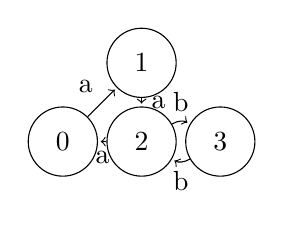
\begin{tikzpicture}[shorten >=1pt,on grid,auto]
        \node[state] (q_0)   {$0$};
        \node[state] (q_1) [above right=of q_0] {$1$};
        \node[state] (q_2) [right=of q_0] {$2$};
        \node[state] (q_3) [right=of q_2] {$3$};
        \path[->]
        (q_0) edge  node {a} (q_1)
        (q_1) edge  node {a} (q_2)
        (q_2) edge  node {a} (q_0)
        (q_2) edge[bend left, above]  node {b} (q_3)
        (q_3) edge[bend left, below]  node {b} (q_2);
        \end{tikzpicture}
        
    \end{center}
    
    Тогда примерами путей, принадлежащих множеству $\Pi = \{\pi \mid \omega(\pi) \in \mathcal{L}\}$, являются:
    
    \begin{center}
        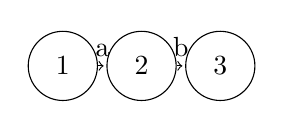
\begin{tikzpicture}[shorten >=1pt,on grid,auto]
        \node[state] (q_1) {$1$};
        \node[state] (q_2) [right=of q_1] {$2$};
        \node[state] (q_3) [right=of q_2] {$3$};
        \path[->]
        (q_1) edge  node {a} (q_2)
        (q_2) edge  node {b} (q_3);
        \end{tikzpicture}
        
    \end{center}
    
    \begin{center}
        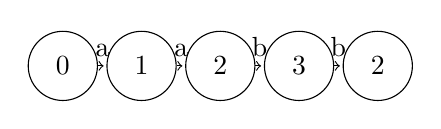
\begin{tikzpicture}[shorten >=1pt,on grid,auto]
        \node[state] (q_0)   {$0$};
        \node[state] (q_1) [right=of q_0] {$1$};
        \node[state] (q_2) [right=of q_1] {$2$};
        \node[state] (q_3) [right=of q_2] {$3$};
        \node[state] (q_4) [right=of q_3] {$2$};
        \path[->]
        (q_0) edge  node {a} (q_1)
        (q_1) edge  node {a} (q_2)
        (q_2) edge  node {b} (q_3)
        (q_3) edge  node {b} (q_4);
        \end{tikzpicture}
        
    \end{center}
    
\end{example}


\section{О разрешимости задачи}

Задачи из определения \ref{def1} и \ref{def2} сводятся к построению пересечения языка $\mathcal{L}$ и языка, задаваемого путями графа, $R$. 
А мы для обсуждения разрешимости задачи рассмотрим более слабую постановку задачи:

\begin{definition}
    Необходимо проверить, что существует хотя бы один такой путь $\pi$ для данного графа, для данного языка $\mathcal{L}$, что $\omega(\pi) \in \mathcal{L}$.
    
\end{definition}

Эта задача сводится к проверке пустоты пересечения языка $\mathcal{L}$ c $R$ --- регулярным языком, задаваемым графом. От класса языка $\mathcal{L}$ зависит её разрешимость:

\begin{itemize}
    \item Если $\mathcal{L}$ регулярный, то получаем задачу пересечения двух регулярных языков: 
    
    $\mathcal{L} \cap R = R'$.
    $R'$ --- также регулярный язык.
    Проверка регулярного языка на пустоту --- разрешимая проблема.
    
    \item Если $\mathcal{L}$ контекстно-свободный, то получаем задачу
    
    $\mathcal{L} \cap R = CF$ --- контекстно-свободный.
    Проверка контекстно-свободного языка на пустоту --- разрешимая проблема.
    
    \item Помимо иерархии Хомского существуют и другие классификации языков.
    Так например, класс конъюнктивных (Conj)
    языков~\cite{DBLP:journals/jalc/Okhotin01}
    является строгим расширением контекстно-свободных языков и все так же позволяет полиномиальный синтаксический анализ.
    
    Пусть $\mathcal{L}$ --- конъюнктивный. При пересечении конъюнктивного и регулярного языков получается конъюнктивный ($\mathcal{L} \cap R = Conj$), а проблема проверки Conj на пустоту не разрешима~\cite{DBLP:journals/tcs/Okhotin03a}.
    
    \item Ещё один класс языков из альтернативной иерархии, не сравнимой с Иерархией Хомского, --- MCFG (multiple context-free grammars)~\cite{SEKI1991191}.
    Как его частный случай --- TAG (tree adjoining grammar)~\cite{Joshi1997}.
    
    Если $\mathcal{L}$ принадлежит классу MCFG, то $\mathcal{L} \cap R$ также принадлежит MCFG. Проблема проверки пустоты MCFG разрешима~\cite{SEKI1991191}.
    
\end{itemize}

Существует ещё много других классификаций языков, но поиск универсальной иерархии до сих пор продолжается.

Далее, для изучения алгоритмов решения, нас будет интересовать задача $R \cap CF$.

\section{Области применения}
\begin{itemize}
    \item Статанализ. 
    Введено Томасом Репсом~\cite{Reps}.
    \item Социальные сети~\cite{Hellings2015PathRF}.
    \item RDF обработка~\cite{10.1007/978-3-319-46523-4_38}.
    \item Биоинформатика~\cite{cfpqBio}.
    \item Применяется для различных межпроцедурных задач~\cite{LabelFlowCFLReachability,specificationCFLReachability,Zheng}.
    \item Графовые БД
    Впервые предложил Михалис Яннакакис~\cite{Yannakakis}.
    
\end{itemize}

\section{Вопросы и задачи}
\begin{enumerate}
    \item Пусть есть граф. Задайте грамматику для поиска всех путей, таких, что....
    \item Существует ли в графе !!! путь из А в Б, такой что!!!
    \item Для графа !!! постройте все пути, удовлетворяющие !!!!
    
    \item Задача 1
    \item Задача 2
\end{enumerate}

\section{Generalized Parser Combinators}
\label{sec:GLL}

Combinators techniques are shown to be applicable for graph traversing~\cite{ScalaGraphParsing}, but it still suffers the common issue with left-recursive definitions.
A general parser combinators library Meerkat~\cite{Meerkat}, implemented in the Scala programming language, removes this restriction by using memoization, continuation-passing style, and the ideas of Johnson~\cite{Johnson}.
It supports the arbitrary (left-recursive and ambiguous) context-free specifications, but it also supports the specification of action code, and provide a \lstinline{syn} macro for custom handling of the recursive nonterminal descriptions.
Meerkat constructs the compact representation of the parse forest in the form of SPPF, which can be used for CFPQs results representation~\cite{GrigorevR16}.
The worst case time and space complexity of the solution is cubic.

%In~\cite{ScalaGraphParsing} showed that combinators techniques is applicable for graph travesing, but well-known problem of combinator with left recursion is not solved.
%But this problew was solved in classical parser-combinators~\cite{Meerkat} and implemented in Meerkat library.
%Meerkat library is a general parser combinators library implemented in Scala programming language; by using memoization, continuation-passing style and the ideas of Johnson~\cite{Johnson}, it supports arbitrary (left-recursive and ambigues) context-free specifications.
%This library implements classical set of combinators, supports action code specification, and provide \lstinline{syn} macro for custom handling of recursive nonterminal description.
%Meercat creates compressed representation of parse forest (SPPF) which is useful for CFPQs results representation~\cite{GrigorevR16}.
%Time and space complexity of this soluton are cubic in worst case.

A Meerkat specification of the language $\{a^n b^n \mid n \geq 1\}$ is presented in fig.~\ref{fig:anbnMeerkat}.

%An example Meerkat specification of grammar~\ref{fig:anbnGrammar} is presented in~\ref{fig:anbnMeerkat}.

\begin{figure}[h]
\begin{lstlisting}
val S = syn("a" ~ S.? ~ "b")
\end{lstlisting}
\caption{Meercat specification of $\{a^n b^n \mid n \geq 1\}$}
\label{fig:anbnMeerkat}
\end{figure}

It is shown in~\cite{GrigorevR16} that Generalized LL parsing algorithm~\cite{scott2010gll} can be generalized to effectively process CFPQs and the query result can be finitely represented.
As the Meerkat library is closely related to the Generalized LL algorithm and since GLL can be generalized for context-free path querying, it is also possible to adapt the Meerkat library for graph querying.
It can be done by providing a function for retrieving the symbols which follow the specified position and utilizing it in the basic set of combinators.
Details are described below.



%In~\cite{GrigorevR16} showed that generalized LL parsing algorithm~\cite{scott2010gll} can be generalized to CFPQs processing and this generalization prodices efficient solution which can provide structured represenataion of query result.
%As the Meerkat library is closely related to the Generalized LL algorithm and since GLL can be generalized for context-free path querying, it is also possible to adapt Meerkat library for graph querying.
%It can be done by providing a function for retrieving the symbols which follow the specified position and utilizing it in the basic set of combinators.
%Details described below.


\subsection{SPPF}

Parsing of a string with respect to an ambiguous grammar can result in several derivation trees for a single string.
The set of derivation trees is named a \emph{derivation forest}.
To store a derivation forest efficiently, the generalized parsing algorithms utilize a \emph{Shared Packed Parse Forest} proposed by Joan Rekers~\cite{SPPF}.
The most efficient compact representation of derivation forests is a Binarized Shared Packed Parse Forest (we will abbreviate it to SPPF)~\cite{brnglr}.
The GLL algorithm, which employs this structure, achieves the worst-case cubic space complexity~\cite{gllParsingTree}.

%Generalized parsing algorithms can handle ambiguose grammars and in this case they produce all posiible derivation trees named dervation forest which can has an exponential size.
%To solve the problem of compact forest representation Shared Packed Parse Forest (SPPF) was proposed by Joan Rekers~\cite{SPPF}.
%Binarized Shared Packed Parse Forest (SPPF)~\cite{brnglr} compresses derivation trees optimally reusing common nodes and subtrees.
%Version of GLL which utilizes this structure for parsing forest representation achieves worst-case cubic space complexity~\cite{gllParsingTree}.

Binarized SPPF is a directed graph, each node of which has one of the four types described below.
Almost every node of the SPPF is decorated with the \emph{extension}: a pair $(i, j)$ where $i$ is a start position of a substring derivable from the node and $j$---its end position.

%Binarized SPPF can be represented as a graph in which each node has one of four types described below.
%We denote the start and the end positions of substring as $i$ and $j$ respectively, and we call tuple $(i,j)$ an \textit{extension} of a node.

\begin{itemize}
    \item \textbf{Terminal node} labelled $(T, i, j)$.
    \item \textbf{Nonterminal node} labelled $(N, i, j)$.
    This node denotes that there is at least one derivation $N \Rightarrow^*_G \omega[i \dots j-1]$---a substring of the input from $i$-th to $j$-th position.
    Every derivation tree for the given substring and nonterminal can be extracted by left-to-right top-down traversal of SPPF started from the respective node.
    \item \textbf{Intermediate node}: a special kind of node used for the binarization of the SPPF. These nodes are labeled with $(t,i,j)$, where $t$ is a grammar slot.
    \item \textbf{Packed node} labelled $(N \rightarrow \alpha, k)$, where $k$ is a position in the input of the right end of leftmost subtree of this node.
    A subgraph with the root in such node is in turn a parse forest for which the first production is $N \rightarrow \alpha$.
%    A subgraph with the ``root'' in such node is one derivation from the nonterminal $N$.

\end{itemize}


An example of SPPF is presented in figure~\ref{fig:sppf}.
We removed redundant intermediate and packed nodes for simplicity and to decrease the size of the figure.

SPPF can finitely represent a possibly infinite set of paths in the context of the language-constrained graph querying~\cite{GrigorevR16}.
Since the SPPF stores derivation trees for all paths, it can be useful for the postprocessing and further understanding of the query results.
In static code analysis, for example, it is possible to map paths back onto the source code thus providing a human-readable result.


%In the context of language-constarined graph querying SPPF can be used as finite represenataion of possibly infinite paths set as showed~\cite{Grigorev16}.
%As far as SPPF stores not only paths but also its derivation trees, this structure may be useful
%for query results understending and postprocessing.
%For example, for static code analysis may be interesting to map path structure to source code in
%order to make results more human-readable.

 \section{Parser Combinators for Path Querying}

Parser combinators provide a way to specify a language syntax in terms of functions and operations on them. 
A parser in this framework is usually a function which consumes a prefix of an input and returns either a parsing result or an error if the input is erroneous. 
Parsers can be composed by using a set of parser combinators to form more complex parsers. 
A parser combinators library provides with a set of basic combinators (such as sequential application or choice), and there can also be user-defined combinators. 
Most parser combinators libraries, including the Meerkat library, can only process the linear input --- strings or some kind of streams. 
We extend the Meerkat library to work on the graph input.

Meerkat library is a general parser combinators library; by using memoization, continuation passing style and the ideas of Johnson~\cite{Johnson} it supports arbitrary context-free specifications. 
As this library is closely related to the Generalized LL algorithm and since GLL can be generalized for context-free path querying~\cite{GrigorevR16}, it is also possible to adapt Meerkat library for graph querying. 
It can be done by providing a function for retrieving the symbols which follow the specified position and utilizing it in the basic set of combinators.

The basic combinators our library provides are presented in table~\ref{table:combinators}. 
Parsers for matching strings are implicitly generated whenever a string is used within a query. 
The classical same generation query~\cite{FndDB} can be written using the library as presented in Fig.~\ref{fig:query1Meerkat}.

\begin{table}[h]
\centering
\begin{tabular}{c|l}
\multicolumn{1}{c|}{Combinator} & \multicolumn{1}{|c}{Description} \\ \hline
{\lstinline!a ~ b!} & sequential parsing: {\lstinline!a!} then {\lstinline!b!}   \\
{\lstinline!a | b!} & choice: {\lstinline!a!} or {\lstinline!b!}         \\
{\lstinline!a.?!}   & optional parsing: {\lstinline!a!} or nothing   \\
{\lstinline!a.*!}   & repetition of zero or more {\lstinline!a!} \\
{\lstinline!a.+!}   & repetition of at least one {\lstinline!a!} \\
\end{tabular}
\caption{Meerkat combinators}
\label{table:combinators}
\end{table}


\begin{figure}[h]
\begin{lstlisting}
val S: Nonterminal = syn(
   "subclassof-1" ~ S.? ~ "subclassof" |
   "type-1" ~ S.? ~ "type")
\end{lstlisting}
\caption{The same generation query (Query 1) in Meerkat}
\label{fig:query1Meerkat}
\end{figure}


The most exciting feature of our library is that queries can be used as first-class values which means greater generalization and composition. 
Function \lstinline{sameGen} presented in Fig~\ref{fig:gen} is a generalization of the same generation query which is independent of the environment such as the input graph structure or other parsers.
It can be used for the creation of other queries, including the one presented in Fig~\ref{fig:query1Meerkat}: it is the result of the application of \lstinline{sameGen} to the appropriate relations (which can be treated as opening and closing brackets).
Another application of the \lstinline{sameGen} can be founded in Fig.~\ref{fig:query2Gen}.

\begin{figure}[h]
\begin{lstlisting}
val query1 = syn(sameGen(List(
    ("subclassof-1", "subclassof"),
    ("type-1", "type"))))
\end{lstlisting}
\caption{Query 1 (Fig.~\ref{fig:query1Meerkat}) as an application of \lstinline{sameGen}}
\label{fig:query1Gen}
\end{figure}

\begin{figure}[h]
\begin{lstlisting}
def sameGen(brs) =
  bs.map { case (lbr, rbr) => 
             lbr ~ syn(sameGen(bs).?) ~ rbr } 
  match {
    case x :: Nil => syn(x)
    case x :: y :: xs => 
      syn(xs.foldLeft(x | y)(_ | _))
  }
\end{lstlisting}
\caption{Generic function for same generations query}
\label{fig:gen}
\end{figure}

Running a query over an input graph retrieves the list of pairs $(i, j)$ where each pair corresponds to the set of paths from the node $i$ to the node $j$. 
Running the same generation query from Fig.~\ref{fig:query2Gen} over the graph in Fig.~\ref{fig:graph} results with $\{(1,0), (1,2)\}$. 
Internally, these paths are represented as SPPF~\cite{SPPF}. 
A simplified SPPF for this query is presented in Fig.~\ref{fig:sppf}: rounded rectangles represent nonterminals and other rectangles represent productions. 
Every rectangle contains a nonterminal name or a production rule, as well as start and end nodes of the path in the input graph derived from the corresponding rectangle. 
Gray rectangles are start nonterminals.

\begin{figure}[h]

\includegraphics[width=0.45\textwidth]{graph}
\caption{Example input graph.}
\label{fig:graph}
\end{figure}

\begin{figure}[h]
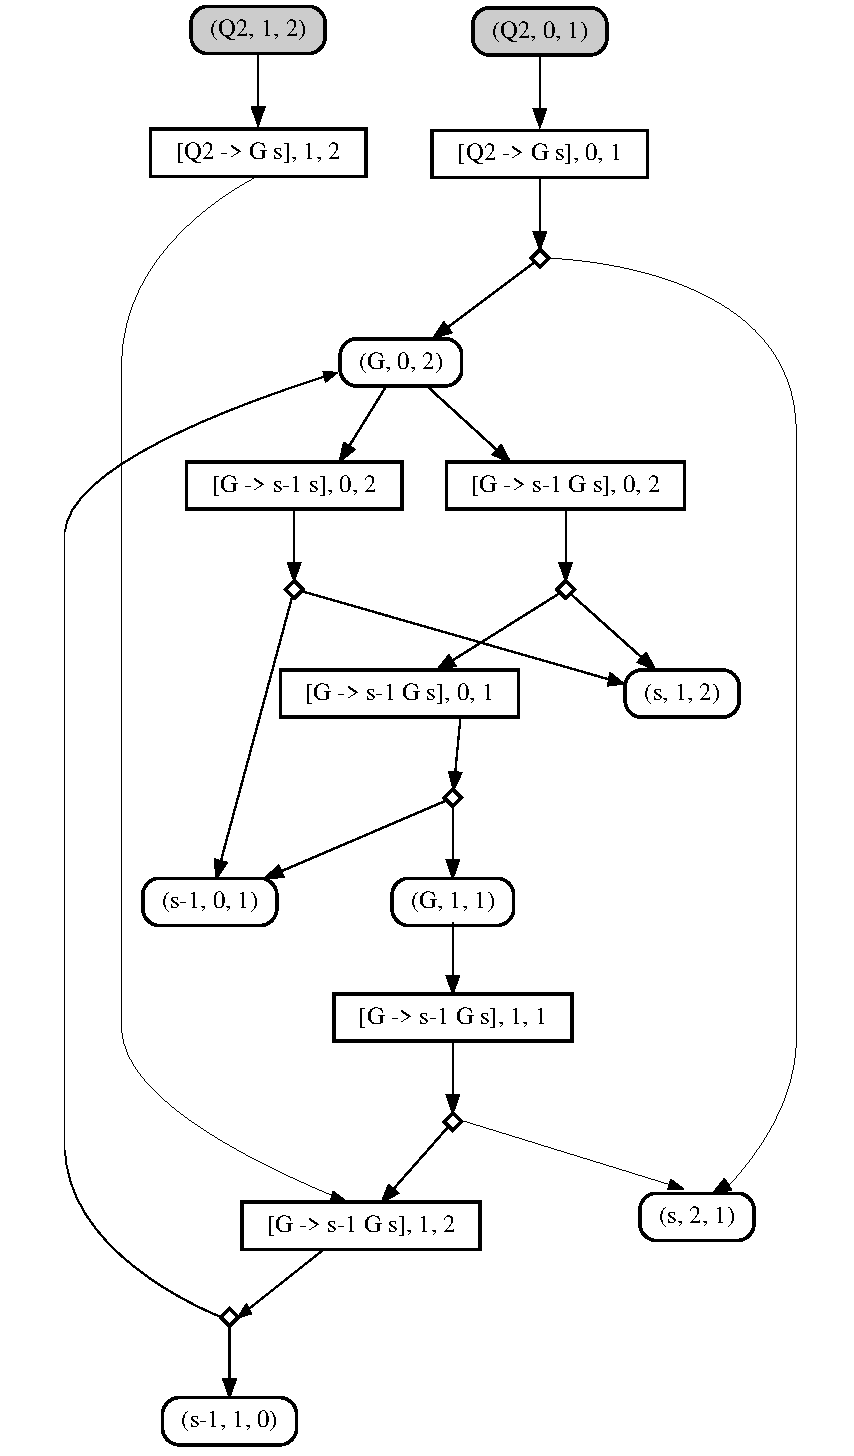
\includegraphics[scale=0.5]{sppf}
\caption{SPPF: result of applying the same generation query~\ref{fig:query2Gen} to the graph~\ref{fig:graph}}
\label{fig:sppf}
\end{figure}

\section{Examples}
\label{sec:examples}

In this section we introduce and describe some examples of our library usage.
We show that combinators are expressive enough for realistic queries and allows to create generic queries easely.

\subsection{Complicated Query to Map}

Let's form a complex query for our city graph. 
Let us capture one city, let's say city with name $a$. 
Now having a city graph and captured vertex we would like to know all paths such if as $i$ city from begining of our path we visit country $X$ then as $i$ city from end of our path we visit country $X$ too. 
And also the middle city in our path is our captured city $a$.
In a terms of combinators we can define our path as shown on fig.~\ref{fig:pathQuery}.
Here \lstinline{reduceChoice} is a function which transforms a list of queries to one query which is formed by reducing given list with \lstinline{|} combinator.
The \lstinline{pathPart} query recursively defines a path of our way.
Also, \lstinline{middleCity} is a vertex query which parses our captured city $a$ and \lstinline{roadTo} query parses a \emph{roadTo} edge.

\begin{figure}[h]
\begin{lstlisting}
val countriesList = List("X", "Y")
val path = 
  (reduceChoice(countriesList.map(pathPart)) | 
    middleCity)
def pathPart(country: String) =
  syn(city(country) ~ roadTo ~ path ~ 
    roadTo ~ city(country))

val middleCity = V(_.value() == "a")
val roadTo = E(_.value() == "road_to")
def city(country: String) =
  V(_.country == country)
\end{lstlisting}
\caption{Path query}
\label{fig:pathQuery}
\end{figure}

\begin{figure}[h]
\begin{lstlisting}
def reduceChoice(xs: List[Nonterminal]) = 
  xs match {
    case x :: Nil     => x
    case x :: y :: xs => 
      syn(xs.foldLeft(x | y)(_ | _))
  }
\end{lstlisting}
\caption{Reduce choice function implementation}
\label{fig:reduceChoice}
\end{figure}

Now we would like, to get from our query only \lstinline{city} combinator result. 
For that purpose let us modify it to make return result. 
In our library we have a \lstinline{^} and \lstinline{&} functions for that. 
Then we will have definition of our combinators as presented in fig.~\ref{fig:fixedPathQ}.

\begin{figure}[h]
\begin{lstlisting}
val middleCity = 
  syn(V(_.value() == "a") ^^) & (List(_))
def pathPart(country: String) = syn(
  (city(country) ~ roadTo ~ 
    path ~ roadTo ~ city(country) & {
      case a ~ (b: List[_]) ~ Entity => 
        a +: b :+ c })
\end{lstlisting}
\caption{Fixed queries}
\label{fig:fixedPathQ}
\end{figure}

Now we execute our query. It is evident that for the graph presented on fig.~\ref{fig:graph} we can get only three paths which satisfies given criteria:
\begin{itemize}
\item single-vertex path $a$;
\item $b \rightarrow a \rightarrow d$
\item $c \rightarrow b \rightarrow a \rightarrow d \rightarrow e$
\end{itemize}

A simplified SPPF for this query is presented in Fig.~\ref{fig:sppf}: rounded rectangles represent nonterminals and other rectangles represent productions. 
Every rectangle contains a nonterminal name or a production rule, as well as start and end nodes of the path in the input graph derived from the corresponding rectangle. 
Gray rectangles are start nonterminals.

\subsection{Same Generation Query}

Yet another example of first order functions usage is generalisation of classical same generation query which is one of basic context-free path queries.
One of application of such queries is hierarchy analysing in RDF storages~\cite{CFGonRDF}.
Let suppose that we have RDF graphs with two pairs of relation (each pair is relation and its revers): (\emph{subClassOf}; $\text{\emph{subClassOf}}^{-1}$) and (\emph{type}; $\text{\emph{type}}^{-1}$).
We want to evaluate two queries which detect all pairs of nodes which are connected by path derivable in grammars $G_1$~(Fig.~\ref{grammarQ1}) and $G_2$ respectively~(Fig.~\ref{grammarQ2}). 


\begin{figure}[h]
   \centering
   \[
\begin{array}{rl}
   0: & S \rightarrow \text{\textit{subClassOf}}^{-1} \ S \ \text{\textit{subClassOf}} \\ 
   1: & S \rightarrow \text{\textit{type}}^{-1} \ S \ \text{\textit{type}} \\ 
   2: & S \rightarrow \text{\textit{subClassOf}}^{-1} \ \text{\textit{subClassOf}} \\ 
   3: & S \rightarrow \text{\textit{type}}^{-1} \ \text{\textit{type}} \\ 
\end{array}
\]
   \caption{Context-free grammar $G_1$ for query 1}
   \label{grammarQ1}
   \end{figure}

\begin{figure}[h]
   \centering
   \[
\begin{array}{rl}
   0: & S \rightarrow B \ \text{\textit{subClassOf}} \\ 
   0: & S \rightarrow \text{\textit{subClassOf}} \\ 
   1: & B \rightarrow \text{\textit{subClassOf}}^{-1} \ B \ \text{\textit{subClassOf}} \\
   2: & B \rightarrow \text{\textit{subClassOf}}^{-1} \ \text{\textit{subClassOf}} \\ 
\end{array}
\]
   \caption{Context-free grammar $G_2$ for query 2}
   \label{grammarQ2}        
   \end{figure}

   Of course, these queries can be written in Meerkat easely because it supports context-free queries: code is presented in Fig.~\ref{fig:query1Meerkat} and Fig.~\ref{fig:query2Meerkat}.

\begin{figure}[h]
\begin{lstlisting}
val query1: Nonterminal = syn(
   "subclassof-1" ~ query1.? ~ "subclassof" |
   "type-1" ~ query1.? ~ "type")
\end{lstlisting}
\caption{The same generation query (Query 1) in Meerkat}
\label{fig:query1Meerkat}
\end{figure}


\begin{figure}[h]
\begin{lstlisting}
val S = syn(
  "subclassof-1" ~ S ~ "subclassof")
val query2 = syn(S ~"subclassof")
\end{lstlisting}
\caption{The same generation query (Query 2) in Meerkat}
\label{fig:query2Meerkat}
\end{figure}

As you can see, grammars and code representations for these two queries looks pretty similar.
May we avoid code duplication and generalize them? 
Yes, we can and not only for these two queries.
The function \lstinline{sameGen} presented in Fig~\ref{fig:gen} is a generalization of the same generation query and is independent of the environment such as the input graph structure or other parsers and also uses a function \lstinline{reduceChoice} presented in \ref{fig:reduceChoice}.
It can be used for the creation of other queries, including the one presented in Fig~\ref{fig:query1Meerkat}: it is the result of the application of \lstinline{sameGen} to the appropriate relations (which can be treated as opening and closing brackets).
Another application of the \lstinline{sameGen} is a Query 2, which can be founded in Fig.~\ref{fig:query2Gen}.


\begin{figure}[h]
\begin{lstlisting}
def sameGen(brs) =
  reduceChoice(
    bs.map { case (lbr, rbr) => 
      lbr ~ syn(sameGen(bs).?) ~ rbr }) 
\end{lstlisting}
\caption{Generic function for the same generations query}
\label{fig:gen}
\end{figure}


\begin{figure}[h]
\begin{lstlisting}
val query1 = syn(sameGen(List(
    ("subclassof-1", "subclassof"),
    ("type-1", "type"))))
\end{lstlisting}
\caption{Query 1 as an application of \lstinline{sameGen}}
\label{fig:query1Gen}
\end{figure}


\begin{figure}[h]
\begin{lstlisting}
val query2 = syn(
  sameGen(List(("subclassof-1", "subclassof"))) ~
   "subclassof")
\end{lstlisting}
\caption{Query 2 as an application of \lstinline{sameGen}}
\label{fig:query2Gen}
\end{figure}


We show that parser combinators provide a simple and safe way to creation of generic queries.
By using this ability, it may be possible to create a library of \ ``standard templates'' for most popular generic queries like same generation query or for domain specific queries (for example, for specific static code analysis problem).


\subsection{Classical Movies Queries}

In order to demonstarte expressive power of our solution and to demonstrate more scenarios for 
semantic actions usage we preovide some examples of classical queries to movie database which 
represents movies, actors, directors, users and relationships between them.
All of queries can be found on a Neo4j tutorial page~\footnote{The set of classical queries to movie dataset in Cypher language: \url{https://neo4j.com/developer/movie-database/}. Access date: 16.01.2018.}.

First of all, we need to introduce some helpers for nodes and edges porcessing simplification.
They are builded upon basic combinators from our library and presented in figure~\ref{fig:helpers}.

\begin{figure}[h]
\begin{lstlisting}
def LV(labels: String*) = V((e: Entity) => labels.forall(e.hasLabel))
def outLE(label: String) = outE((e: Entity) => e.label() == label)
def inLE(label: String) = inE((e: Entity) => e.label() == label)
\end{lstlisting}
\caption{Helpers for edges and nodes processing}
\label{fig:helpers}
\end{figure}

\begin{figure}[h]
\begin{lstlisting}

val query = syn((LV("Movie") :: V((_:Entity).title == "Forrest Gump")) ~ inLE("ACTS_IN") ~
                      syn(LV("Actor") ^ (_.getProperty[String]("name"))) &&)

    executeQuery(query, input).foreach(println)



    ========================
val query = syn((syn(LV("Actor") ^^) ~ outLE("ACTS_IN") ~ LV("Movie")) &
      ((a: Entity) => (a.getProperty[String]("name"), a.id.asInstanceOf[String].toInt)))

    executeQuery(query, input)
      .groupBy({case (a, i) => i})
      .toIndexedSeq
      .map({case (i, ms) => (ms.head._1, ms.length)})
      .sortBy({case (a, mc) => -mc})
      .take(10)
      .foreach({case (a, mc) => println(a, mc)})


==========================

val directors = syn((syn(LV("Actor", "Director") ^^) ~ outLE("Directed") ~ LV("Movie"))
                    & (d  => d.id.asInstanceOf[String].toInt))

    val directorsMap = executeQuery(directors, input)
      .groupBy(i => i)
      .map({case (i, ms) => (i, ms.length)})
      .filter({case (_, ms) => ms >= 2})

    val actor_prof_director = syn(LV("Actor", "Director") :: V((e: Entity) => directorsMap.contains(e.id.asInstanceOf[String].toInt)) ^^)

    val acts = syn((actor_prof_director ~ outLE("ACTS_IN") ~ LV("Movie")) &
      (a => (a.getProperty[String]("name"), a.id.asInstanceOf[String].toInt)))

    executeQuery(acts, input)
      .groupBy({case (a, i) => i})
      .toStream
      .map({case (i, ms) => (i, ms.head._1, ms.length)})
      .filter({case (i, a, mc) => mc >= 10})
      .foreach({case (i, a, mc) => println((a, mc, directorsMap(i)))})

===========================================

    val adilfulara = syn(LV("User") :: V((_: Entity).login == "adilfulara"))

    val query = syn((adilfulara ~ (outLE("FRIEND") | inLE("Friend")) ~ syn(LV("Person") ^^) ~
                                 syn(outLE("RATED") ^^) ~ syn(LV("Movie") ^^)) &
      {case p ~ r ~ m => (p.getProperty[String]("name"), m.title, r.stars.asInstanceOf[Int],
                          if (r.hasProperty("comment")) r.comment else "")})

    executeQuery(query, input)
      .filter({case (_, _, s, _) => s > 3})
      .foreach(println)


      =======================================

      MATCH (m:Movie {title: 'Forrest Gump'})<-[:ACTS_IN]-(a:Actor)

RETURN a.name, a.birthplace
======================
MATCH (a:Actor)-[:ACTS_IN]->(m:Movie)

RETURN a, count(*)

ORDER BY count(*) DESC LIMIT 10;
================================
MATCH (a:Actor)-[:ACTS_IN]->(m:Movie)

WITH a, count(m) AS acted

WHERE acted >= 10

WITH a, acted

MATCH (a:Director)-[:DIRECTED]->(m:Movie)

WITH a, acted, collect(m.title) AS directed

WHERE length(directed) >= 2

RETURN a.name, acted, directed

ORDER BY length(directed) DESC, acted DESC;
\end{lstlisting}
\caption{Mutual Friend recommendations query in Cypher}
\label{fig:cypher_movie_query}
\end{figure}


Let's look at one of these examples written using Cypher language and how it transforms into Meerkat query
(fig.~\ref{fig:cypher_movie_query}).

\begin{figure}[h]
\begin{lstlisting}
MATCH (u:User {login: 'adilfulara'})-[:FRIEND]->
      (f:Person)-[r:RATED]->(m:Movie)
WHERE r.stars > 3
RETURN f.name, m.title, r.stars, r.comment
\end{lstlisting}
\caption{Mutual Friend recommendations query in Cypher}
\label{fig:cypher_movie_query}
\end{figure}

Firstly, we should define parsers that correspond to persons, movies and specific user.
Secondly, we should also create parsers corresponding to relations.
Then, we can get a full path parser using combination of previously defined primitives.
Finally, adding semantic action that extracts all needed data we get a complete path query.
Result is shown on fig.~\ref{fig:meerkat_movie_query}.
Using similar transformations we can write the most queries which can be defined using Cypher.


\begin{figure}[h]
\begin{lstlisting}
val adilfulara = 
    syn(V((e: Entity) => e.hasLabel("User") 
                && e.login == "adilfulara"))
val friend = 
    syn(E((e: Entity) => e.value() == "FRIEND"))

val person = 
    syn(V((e: Entity) => e.hasLabel("Person")) ^^)

val rated = 
    syn(E((e: Entity) => e.value() == "RATED") ^^)

val movie = 
    syn(V((e: Entity) => e.hasLabel("Movie")) ^^)

val query = 
    syn((adilfulara ~ friend ~ person ~ 
         rated ~ movie) &
    {case p ~ r ~ m => 
        (p.name, m.title, r.stars.asInstanceOf[Int],
         if (r.hasProperty("comment")) r.comment 
         else "")})

executeQuery(query, input)
  .filter({case (_, _, s, _) => s > 3})
\end{lstlisting}
\caption{Mutual Friend recommendations (Meerkat query)}
\label{fig:meerkat_movie_query}
\end{figure}

We show that our library is expressive enough to fromulate realistic queries. 
Also we demonstrate some cases of semantics actions usage.
Main difference from Cypher is that library provides only path querying mechanusms, so all additional logic such as
filtering, sorting or grouping must be implemented manually as a separated step.

Also, we detect that our library doesn't support incoming edges precessing which may be useful in some scenarios.
\section{Evaluation}

We evaluate the implemented algorithm on both regular and context-free path queries in order to demonstrate applicability of the proposed solution.
Namely, goals of the evaluation are following.
\begin{enumerate}
	\item Investigate the practical applicability of RPQ evaluation by the proposed algorithm.
	\item Compare Azimov's algorithm for reachability CFPQ and the proposed algorithm.
	\item Investigate the practical applicability of paths extraction algorithm for both regular and context-free queries.
\end{enumerate}

For evaluation, we use a PC with Ubuntu 18.04 installed.
It has Intel core i7-6700 CPU, 3.4GHz, and DDR4 64Gb RAM.
As far as we evaluate only algorithm execution time, we store each graph fully in RAM as its adjacency matrix in sparse format.
Note, that graph loading time is not included in the result time of evaluation.	

\subsection{RPQ Evaluation}

In oder to investigate applicability of the proposed algorithm for RPQ over real-world graphs we collect a set of real-world and synthetic graphs and evaluate queries generated by using the most popular templates for RPQs.

\subsubsection{Dataset}

Brief description of collected graphs are presented in Table~\ref{tbl:graphs_for_rpq}.
Namely, the dataset consists of several parts.
The first one is a set of LUBM graphs\footnote{Lehigh University Benchmark (LUBM) web page: \url{http://swat.cse.lehigh.edu/projects/lubm/}. Access date: 07.07.2020.}~\cite{10.1016/j.websem.2005.06.005} with a different number of vertices.
The second one is a graphs from Uniprot database\footnote{Universal Protein Resource (UniProt) web page: \url{https://www.uniprot.org/}. All files used for evaluation can be downloaded here: \url{ftp://ftp.uniprot.org/pub/databases/uniprot/current_release/rdf/}. Access date: 07.07.2020.}: \textit{proteomes}, \textit{taxonomy} and \textit{uniprotkb}.
The last part is a RDF files \textit{mappingbased\_properties} from DBpedia\footnote{DBpedia project web site: \url{https://wiki.dbpedia.org/}. Access date: 07.07.2020.} and \textit{geospecies}\footnote{The Geospecies RDF: \url{https://old.datahub.io/dataset/geospecies}. Access date: 07.07.2020.}.
These graphs represent data from different areas and they are frequently used for graph querying algorithms evaluation.

\begin{table}
{
\rowcolors{2}{black!2}{black!10}
\begin{tabular}{|l|c|c|}
\hline
Graph & \#V & \#E \\
\hline
\hline 
LUBM1k  & 120 926 & 484 646 \\
LUBM3.5k  & 358 434 & 144 9711 \\
LUBM5.9k  & 596 760 & 2 416 513 \\
LUBM1M   & 1 188 340 & 4 820 728 \\
LUBM1.7M & 1 780 956 & 7 228 358 \\
LUBM2.3M & 2 308 385 & 9 369 511 \\
\hline
Uniprotkb & 6 442 630 & 24 465 430 \\
Proteomes & 4 834 262 & 12 366 973 \\
Taxonomy & 5 728 398 & 14 922 125 \\
\hline
Geospecies & 450 609 & 2 201 532 \\
Mappingbased\_properties & 8 332 233 & 25 346 359 \\
\hline
\end{tabular}
}
\caption{Graphs for RPQ evaluation}
\label{tbl:graphs_for_rpq}
\end{table}


Queries for evaluation was generated by using templates of the most popular RPQs which are collected from~
\cite{Pacaci2020RegularPQ} (Table 2) and~\cite{Wang2019} (some of complex queries from Table 5), and are presented in table~\ref{tbl:queries_templates}.
We generate 10 queries for each template and each graph using the most frequent relations from the given graph randomly\footnote{Used generator is available as part of CFPQ\_data project: \url{https://github.com/JetBrains-Research/CFPQ_Data/blob/master/tools/gen_RPQ/gen.py}. Access data: 07.07.2020.}. 
For all LUBM graphs common set of queries was generated in order to investigate scalability of the proposed algorithm.

\begin{table}
{\small
\renewcommand{\arraystretch}{1.25}
\rowcolors{2}{black!2}{black!10}
\begin{tabular}{|c|c||c|c|}
\hline

Name & Query & Name & Query \\
\hline
\hline 
$Q_1$   & $a^*$                               & $Q_9^5$    & $(a \mid b \mid c \mid d \mid e)^+$                     \\
$Q_2$   & $a\cdot b^*$                        & $Q_{10}^2$ & $(a \mid b) \cdot c^*$                                  \\
$Q_3$   & $a \cdot b^* \cdot c^*$             & $Q_{10}^3$ & $(a \mid b \mid c)  \cdot d^*$                          \\
$Q_4^2$ & $(a \mid b)^*$                      & $Q_{10}^4$ & $(a \mid b \mid c \mid d)  \cdot e^*$                   \\
$Q_4^3$ & $(a \mid b \mid c)^*$               & $Q_{10}^5$ & $(a \mid b \mid c \mid d \mid e)  \cdot f^*$            \\
$Q_4^4$ & $(a \mid b \mid c \mid d)^*$        & $Q_{10}^2$ & $a \cdot b$                                             \\
$Q_4^5$ & $(a \mid b \mid c \mid d \mid e)^*$ & $Q_{11}^3$ & $a \cdot b \cdot c$                                     \\
$Q_5$   & $a \cdot b^* \cdot c$               & $Q_{11}^4$ & $a \cdot b \cdot c \cdot d$                             \\
$Q_6$   & $a^* \cdot b^*$                     & $Q_{11}^5$ & $a \cdot b \cdot c \cdot d \cdot f$                     \\
$Q_7$   & $a \cdot b \cdot c^*$               & $Q_{12}$   & $(a \cdot b)^+ \mid  (c \cdot d)^+$                     \\
$Q_8$   & $a? \cdot b^*$                      & $Q_{13}$   & $(a \cdot(b \cdot c)^*)^+ \mid  (d \cdot f)^+$          \\
$Q_9^2$ & $(a \mid b)^+$                      & $Q_{14}$   & $(a \cdot b \cdot (c \cdot d)^*)^+  \cdot (e \mid f)^*$ \\
$Q_9^3$ & $(a \mid b \mid c)^+$               & $Q_{15}$   & $(a \mid b)^+ \cdot (c \mid d)^+$                       \\
$Q_9^4$ & $(a \mid b \mid c \mid d)^+$        & $Q_{16}$   & $a \cdot b \cdot (c \mid d \mid e)$                     \\
\hline
\end{tabular}
}
\caption{Queries' templates for RPQ evaluation}
\label{tbl:queries_templates}
\end{table}


\subsubsection{Results}

For reachability index creation average time of 5 runs is presented.

Reachability index creation time for each query for LUBM graphs set is presented in figure~\ref{fig:lubm_all_qs}.
We can observe linear !!!! dependency of evaluation time on graph size.
Also we can see, that query evaluation time depends on query: there are queries which evaluate less then 1 second even for biggest graph ($Q_2$, $Q_5$, $Q_{11}^2$, $Q_{11}^3$), while worst time is 6.26 seconds ($Q_{14}$).
Anyway, we can argue that in this case our algorithm demonstrates reasonable time to be applied for real-world data analysis, because it is comparable with recent results on the same problem for LUBM querying by using distributed system over 10 nodes~\cite{Wang2019}, while we use only one node. 
Note, that accurate comparison of different approaches is a huge interesting work for the future.

\begin{figure}
   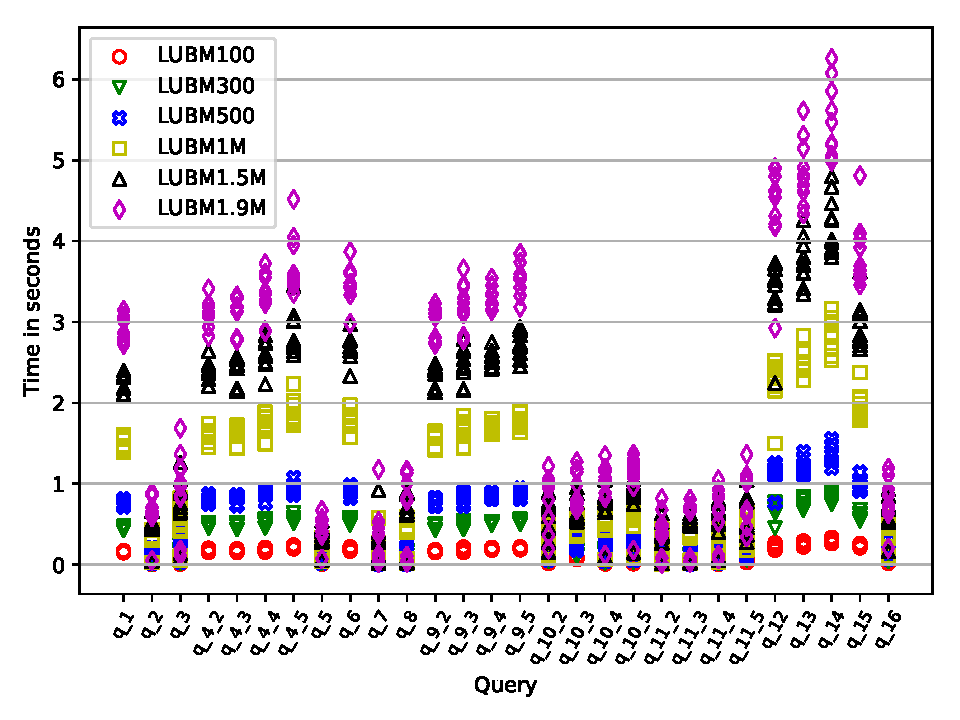
\includegraphics[width=0.48\textwidth]{data/LUBM_all.pdf}
   \caption{Reachability index creation time for LUBM graphs}
   \label{fig:lubm_all_qs}
\end{figure}

Reachability index creation time for each query for for real-world graphs is presented in figure~\ref{fig:other_all_qs}.
We can see that query evaluation time depends on graph inner structure. 
First of all, in some cases handling of small graph requires more time, then handling bigger graph.
For example, $Q_{10}^4$: querying the \textit{geospecies} graph (450k vertices) in some cases requires more time than querying of \textit{mappingbased\_properties} (8.3M vertices) and \textit{taxonomy} (5.7M vertices).
On the other hand, \textit{taxonomy} querying in relatively big number of cases requires significantly more time, than querying of other graphs, while \textit{taxonomy} is not a biggest graph. 
Finally, we can see, that in big number of cases query execution time requires less then 10 seconds, even for big graph, and no queries which require more then 52.17 seconds. 

\begin{figure}
   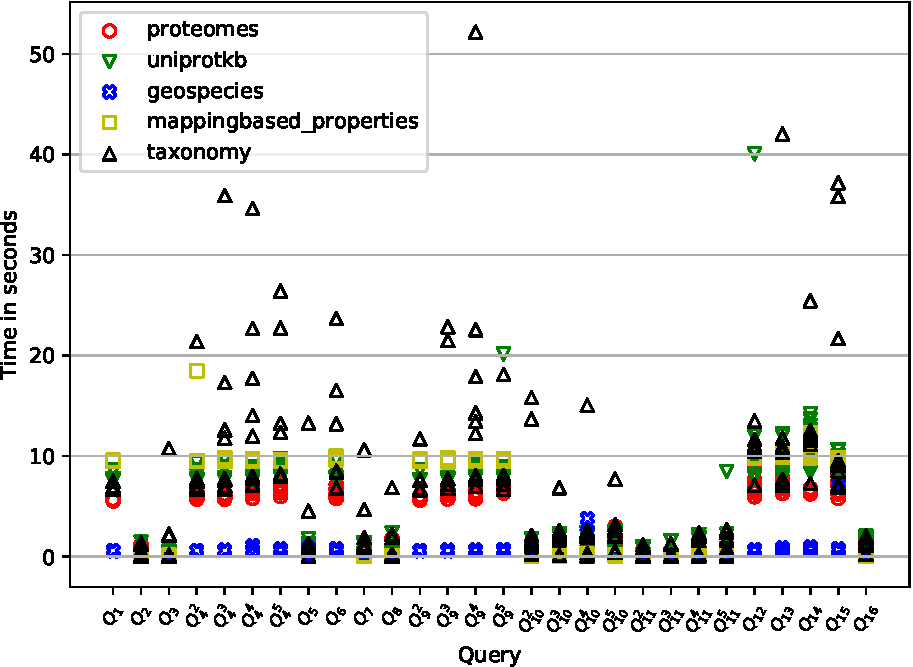
\includegraphics[width=0.48\textwidth]{data/other_all.pdf}
   \caption{Reachability index creation time for real-world RDFs}
   \label{fig:other_all_qs}
\end{figure}

Paths extraction was evaluated on cases with possible long paths.
These cases were selected during reachability index creation by using number of iterations in transitive closure evaluation.
For each selected graph and query we measure paths extraction time for each reachable pair, reachability index creation time is not included because exactly the same index, as calculated at the previous step, is used for paths extraction. 

We evaluate two scenarios.
The first one is a single path extraction.
In this case results are represented as a dependency of extraction time on extracted path length.
We can see linear !!!!

The second scenario is many paths extraction.
Here we limit a number of path to extract by !!! 
In this case results are represented as a dependency of extraction time on number of extracted paths.


\begin{figure}
     \begin{subfigure}[b]{0.24\textwidth}
         \centering
         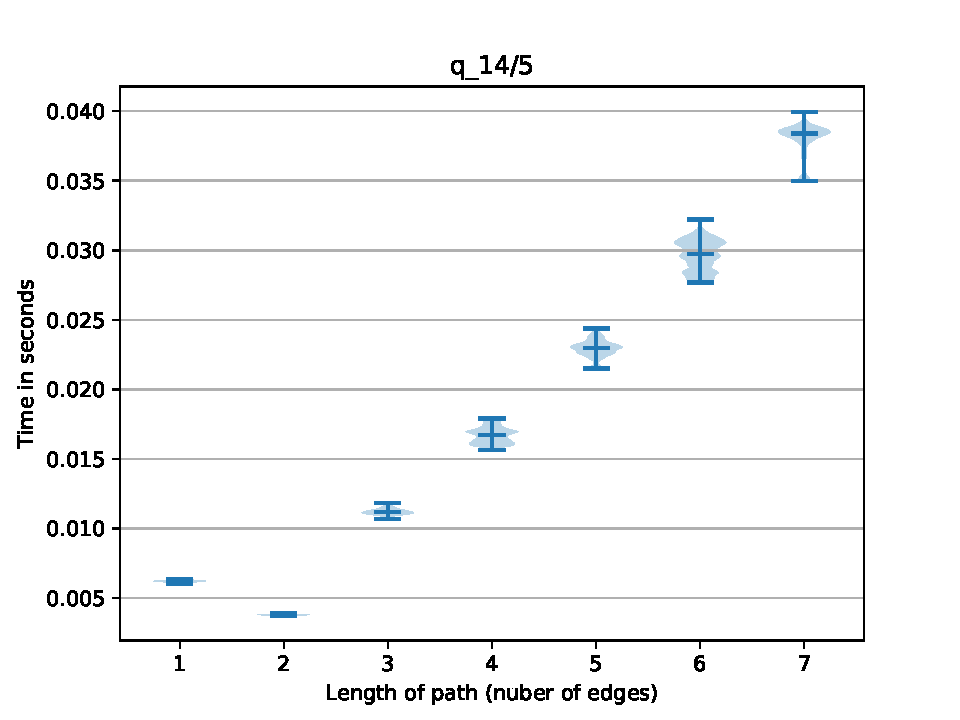
\includegraphics[width=\textwidth]{data/res_graphics/q_14_5.pdf}
         \caption{$y=x$}
         \label{fig:y equals x}
     \end{subfigure}
     ~\begin{subfigure}[b]{0.24\textwidth}
         \centering
         %\includegraphics[width=\textwidth]{data/res_graphics/q9_2_8.pdf}
         \caption{$y=x$}
         \label{fig:y equals x}
     \end{subfigure}\\
     \begin{subfigure}[b]{0.24\textwidth}
         \centering
         %\includegraphics[width=\textwidth]{data/res_graphics/q_14_8.pdf}
         \caption{$y=x$}
         \label{fig:y equals x}
     \end{subfigure}
     ~\begin{subfigure}[b]{0.24\textwidth}
         \centering
         %\includegraphics[width=\textwidth]{data/res_graphics/q4_2_8.pdf}
         \caption{$y=x$}
         \label{fig:y equals x}
     \end{subfigure}
   %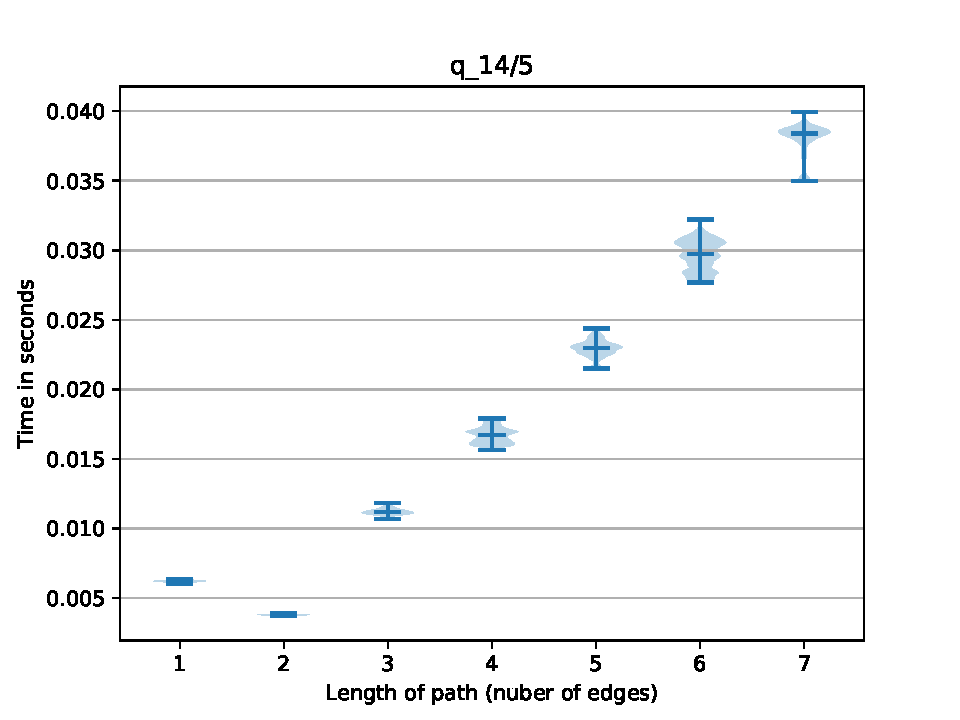
\includegraphics[width=0.48\textwidth]{data/res_graphics/q_14_5.pdf}
   \caption{Single path extraction}
\end{figure}

\subsubsection{Conclusion}

We can conclude that proposed algorithm is applicable for real-world data processing: the algorithm allows one both to solve reachability problem and to extract paths of interest in reasonable time even using na{\"i}ve implementation.  

\subsection{CFPQ Evaluation}

Comparison with matrix-based algorithm.

\subsubsection{Dataset}

Dataset for evaluation. 
It should be CFPQ\_Data\footnote{CFPQ\_Data is a dataset for CFPQ evaluation which contains both synthetic and real-world data and queries \url{https://github.com/JetBrains-Research/CFPQ\_Data}. Access date: 07.07.2020.}

\begin{table}
{
\rowcolors{2}{black!2}{black!10}
\begin{tabular}{|l|c|c|}
\hline
Graph & \#V & \#E \\
\hline
\hline 
eclass\_514en  & 120 926 & 484 646 \\
enzyme  & 358 434 & 144 9711 \\
geospecies  & 596 760 & 2 416 513 \\
go   & 1 188 340 & 4 820 728 \\
go-hierarchy & 1 780 956 & 7 228 358 \\
taxonomy & 2 308 385 & 9 369 511 \\
\hline
Aliases 1 & 6 442 630 & 24 465 430 \\
Aliases 2 & 4 834 262 & 12 366 973 \\
.... & 5 728 398 & 14 922 125 \\
\hline
\end{tabular}
}
\caption{Graphs for CFPQ evaluation}
\label{tbl:graphs_for_cfpq}
\end{table}



Same-generation queries, memory aliases.

\subsubsection{Results}

Results of evaluation.

Index creation.

{\setlength{\tabcolsep}{0.4em}
	\begin{table}
		\caption{RDFs query $G_1$ and $G_2$ (time is measured in seconds and memory is measured in megabytes)}
		\label{tbl:tableRDFQ1_appendix}
		\rowcolors{4}{black!2}{black!10}
		\small
		\begin{tabular}{| l | c | c | c | c |}
			\hline
			
			\multirow{2}{*}{Name}  & \multicolumn{2}{c|}{$G_1$} & \multicolumn{2}{c|}{$G_2$} \\
			\cline{2-5}
			                       & Tensors & RG\_CPU\textsubscript{path} & Tensors & RG\_CPU\textsubscript{path}	 \\
			\hline
			\hline
			eclass\_514en   & 0.254   & 0.195   & 0.227 & ...\\
			enzyme          & 0.035   & 0.029   & 0.036 & ...\\
			geospecies      & 0.091   & ...     & 0.001 & ...\\
			go-hierarchy    & 0.186   & 0.976   & 0.293 & ...\\
			go              & 1.676   & 1.286   & 1.368 & ...\\
			pathways        & 0.015   & 0.021   & 0.009 & ...\\
			taxonomy        & 5.366   & .....   & 3.282 & ...\\
			\hline
		\end{tabular}
	\end{table}
}


Paths extraction.

\subsubsection{Conclusion}

\section{Conclusion and future work}
In this paper, we shown how the context-free path query evaluation w.r.t. the relational and the single-path query semantics can be reduced to the calculation of matrix transitive closure. Also, we provided a formal proof of the correctness of the proposed reduction. In addition, we introduced an algorithm for computing this transitive closure, which allows us to efficiently apply GPGPU computing techniques. Finally, we shown the practical applicability of the proposed algorithm by running different implementations of our algorithm on real-world data.

We can identify several open problems for further research. In this paper we have considered only two semantics of context-free path querying but there are other important semantics, such as all-path query semantics~\cite{hellingsPathQuerying} which requires to present all paths for all triples $(A,m,n)$. Context-free path querying implemented with algorithm~\cite{GLL} can answer the queries in all-path query semantics by constructing a parse forest. It is possible to construct a parse forest for a linear input by matrix multiplication~\cite{okhotin_cyk}. Whether it is possible to generalize this approach for a graph input is an open question.

In our algorithm, we calculate the matrix transitive closure naively, but there are algorithms for the transitive closure calculation, which are asymptotically more efficient. Therefore, the question is whether it is possible to apply these algorithms for the matrix transitive closure calculation to the problem of context-free path querying.

Also, there are Boolean grammars~\cite{okhotinBoolean}, which have more expressive power than context-free grammars. Boolean path querying is an undecidable problem~\cite{hellingsRelational} but our algorithm can be trivially generalized to work on boolean grammars because parsing with boolean grammars can be expressed by matrix multiplication~\cite{okhotin_cyk}. It is not clear what a result of our algorithm applied to Boolean grammars would look like. Our hypothesis is that it would produce the upper approximation of a solution.

From a practical point of view, matrix multiplication in the main loop of the proposed algorithm may be performed on different GPGPU independently. It can help to utilize the power of multi-GPU systems and increase the performance of context-free path querying.

There is an algorithm~\cite{apspGPU} for transitive closure calculation on directed graphs which generalized to handle graph sizes inherently larger then the DRAM memory available on the GPU. Therefore, the question is whether it is possible to apply this approach to the matrix transitive closure calculation in the problem of context-free path querying.

\section*{Acknowledgments}

The research was supported by the Russian Science Foundation grant 18-11-00100 and a grant from JetBrains Research.

\bibliographystyle{ACM-Reference-Format}
\bibliography{combinators_for_graph_querying}

\end{document}
